\chapter{Market Microstructure}
\label{ch:microstructure}

\begin{companioncode}{quant-microstructure}
Code: \texttt{crates/quant-microstructure/}\\
Dependencies: \crate{quant-core}, \crate{thiserror}\\
Run: \texttt{cargo run -p quant-microstructure --example lob\_demo}\\
Run: \texttt{cargo run -p quant-microstructure --example ofi\_demo}
\end{companioncode}

\section{Learning Objectives}

This chapter moves from the daily/return horizon of portfolio theory
into the intraday world of the limit order book (LOB). After completing
it you can:

\begin{itemize}
    \item Represent a limit order book with price-time priority using
      integer tick prices and a \texttt{BTreeMap} keyed by price level
    \item Implement the three core operations --- add, cancel, market
      order --- and reason about their complexity
    \item Compute the order flow imbalance (OFI) series from a sequence
      of book snapshots
    \item Compute volume-weighted average price (VWAP) from fills and
      trade imbalance from signed trades
    \item Apply the square-root (Almgren-Chriss) and linear market
      impact models to estimate the cost of executing a market order
    \item Combine half-spread and impact into a single execution-cost
      estimate in basis points
\end{itemize}

\begin{keyinsight}
Microstructure is where the frictionless world of Markowitz meets
reality. The bid-ask spread is the price of immediacy: takers pay it,
makers earn it. The square-root impact law says that moving size
$Q$ through the market costs $\sigma\sqrt{Q/V}$ in fraction of price
--- a non-linear function of participation rate. Together, spread
plus impact turn the efficient frontier into a \emph{reachable}
frontier net of trading costs.
\end{keyinsight}

\section{Why Microstructure Matters}

The portfolio theory of \cref{ch:portfolio} assumes frictionless
trading: you can rebalance to the tangency portfolio at no cost. In
reality every trade pays the half-spread and pushes the price against
itself. The combined cost is small for a retail order of 100 shares,
but it dominates the economics of executing a $\$100$M rebalance.

Market microstructure studies the mechanism by which trades occur and
how that mechanism affects price formation. Three quantities capture
most of the relevant friction:

\begin{enumerate}
    \item \textbf{The bid-ask spread} --- the difference between the
      best (lowest) ask and the best (highest) bid. A market taker
      buys at the ask and sells at the bid, paying the full spread;
      the maker on the other side earns half of it on average.
    \item \textbf{Market impact} --- the adverse price move caused by
      your own order. A large buy lifts the ask; subsequent fills
      happen at worse prices. Empirically the impact scales as the
      square root of the order size relative to daily volume.
    \item \textbf{Order flow imbalance (OFI)} --- a signed measure of
      buying versus selling pressure at the top of the book. Positive
      OFI predicts positive short-horizon returns.
\end{enumerate}

\section{The Limit Order Book}

A limit order book aggregates all outstanding resting orders. Each
order has a side (bid or ask), a price, a quantity, and a timestamp.
Orders at the same price execute in \emph{price-time priority}: the
best price first, and at that price, the earliest timestamp first
(FIFO).

We represent prices as integer ticks (\texttt{u64}) to avoid
floating-point comparison issues. A tick size of 1 means one unit of
price (e.g.\ one cent); a tick size of 10 means prices must be
multiples of 10. The book stores bids and asks in two
\texttt{BTreeMap<u64, Vec<Order>>} keyed by price. For bids, the best
(highest) price is the last key; for asks, the best (lowest) price is
the first key. A \texttt{HashMap<order\_id, (side, price)>} index
gives $O(1)$ cancel lookup.

\vspace{-2cm}
\marginnote{%
\textbf{Why integer ticks?}\\[0.3em]
Float comparison is non-associative and rounding-dependent. The book
must compare prices \emph{exactly}: an order either matches the tick
grid or it does not. \texttt{u64} ticks make that comparison trivial
and unambiguous.
}

\marginnote{%
\textbf{BTreeMap per side}\\[0.3em]
A \texttt{BTreeMap<u64, \_>} gives ordered price levels with
$O(\log L)$ insert and best-price lookup. The price \emph{is} the key,
so the book never has to sort --- ordering is structural. A
\texttt{HashMap} would not preserve order; a sorted \texttt{Vec} would
shift data on every insert.
}

\begin{marginfigure}
    \centering
    \vspace{-1cm}
    % Limit order book depth diagram.
% Horizontal bars: each price level is one row, bar length = quantity.
% Asks (sellers) above in red, bids (buyers) below in blue. The spread
% is the gap between best bid (100) and best ask (101).

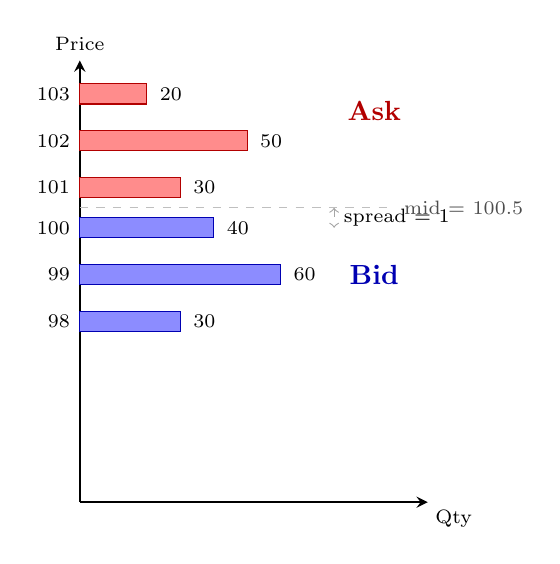
\begin{tikzpicture}[
    scale=0.85,
    every node/.style={font=\scriptsize},
    bidbar/.style={fill=blue!45, draw=blue!70!black},
    askbar/.style={fill=red!45,  draw=red!70!black},
]

% Axes
\draw[->, thick, >=stealth] (0,0) -- (5.2,0) node[below right=-1pt] {Qty};
\draw[->, thick, >=stealth] (0,0) -- (0,6.6) node[above] {Price};

% Asks (descending from best ask at 101, drawn above the mid line)
%   y-position chosen so each level sits on its own row
\node[left] at (0, 6.10) {103};
\filldraw[askbar] (0, 5.95) rectangle (1.0, 6.25);
\node[right] at (1.05, 6.10) {20};

\node[left] at (0, 5.40) {102};
\filldraw[askbar] (0, 5.25) rectangle (2.5, 5.55);
\node[right] at (2.55, 5.40) {50};

\node[left] at (0, 4.70) {101};
\filldraw[askbar] (0, 4.55) rectangle (1.5, 4.85);
\node[right] at (1.55, 4.70) {30};

% Spread annotation between best ask (101) and best bid (100)
\draw[<->, dashed, gray!70] (3.8, 4.40) -- (3.8, 4.10);
\node[right] at (3.8, 4.25) {spread = 1};

% Bids (descending from best bid at 100, drawn below the mid line)
\node[left] at (0, 4.10) {100};
\filldraw[bidbar] (0, 3.95) rectangle (2.0, 4.25);
\node[right] at (2.05, 4.10) {40};

\node[left] at (0, 3.40) {99};
\filldraw[bidbar] (0, 3.25) rectangle (3.0, 3.55);
\node[right] at (3.05, 3.40) {60};

\node[left] at (0, 2.70) {98};
\filldraw[bidbar] (0, 2.55) rectangle (1.5, 2.85);
\node[right] at (1.55, 2.70) {30};

% Mid price dashed line
\draw[dashed, gray!50] (0, 4.40) -- (4.7, 4.40);
\node[right, gray!60!black] at (4.7, 4.40) {mid = 100.5};

% Side labels
\node[red!70!black,  font=\bfseries] at (4.4, 5.85) {Ask};
\node[blue!70!black, font=\bfseries] at (4.4, 3.40) {Bid};

\end{tikzpicture}
    \caption{Resting depth at three price levels on each side. Best
    bid at 100 (40 shares), best ask at 101 (30 shares), spread = 1,
    mid = 100.5.}
    \label{fig:lob-depth}
\end{marginfigure}

\subsection{Core Types}

The basic types are intentionally small and \texttt{Copy} where
possible so that the book can pass them by value without ceremony.

\begin{lstlisting}[caption={Core microstructure types}]
pub enum Side { Bid, Ask }

pub struct Order {
    pub id: u64,
    pub side: Side,
    pub price: u64,
    pub quantity: u64,
    pub timestamp: u64,
}

pub struct Level {
    pub price: u64,
    pub quantity: u64,
    pub order_count: usize,
}

pub struct Fill {
    pub price: u64,
    pub quantity: u64,
    pub maker_order_id: u64,
}
\end{lstlisting}

\subsection{Adding and Cancelling Orders}

\marginnote{%
\textbf{Price-time priority}\\[0.3em]
Orders at the same price execute in FIFO order: the earliest
timestamp fills first. At each price level we store orders in a
\texttt{Vec} in insertion order, and market orders consume the front
of the vector. Time is secondary to price --- a worse-priced order
never jumps ahead of a better one, regardless of age.
}

\func{add\_order} validates that the price is a multiple of the tick
size, that the quantity is positive, and that the order id is unique.
It then inserts the order at the back of the vector for its price
level and records the id in the index.

\func{cancel\_order} looks up the (side, price) pair in the index,
finds the order in the level's vector, removes it, and prunes the
level if it becomes empty. Both operations are $O(\log L + K)$ where
$L$ is the number of price levels and $K$ is the number of orders at
that level; the index makes cancel $O(1)$ to locate the level.

\begin{lstlisting}[caption={Adding a limit order}]
pub fn add_order(&mut self, order: Order) -> Result<(), MicroError> {
    if self.tick_size > 0 && order.price % self.tick_size != 0 {
        return Err(MicroError::InvalidOrder(format!(
            "price {} is not a multiple of tick size {}",
            order.price, self.tick_size
        )));
    }
    if order.quantity == 0 {
        return Err(MicroError::InvalidOrder("quantity must be positive".into()));
    }
    if self.index.contains_key(&order.id) {
        return Err(MicroError::InvalidOrder(format!(
            "duplicate order id {}", order.id
        )));
    }
    self.index.insert(order.id, (order.side, order.price));
    let book = match order.side {
        Side::Bid => &mut self.bids,
        Side::Ask => &mut self.asks,
    };
    book.entry(order.price).or_insert_with(Vec::new).push(order);
    Ok(())
}
\end{lstlisting}

\subsection{Market Orders and Price-Time Priority}

A market order has no price: it takes liquidity from the opposite side
until filled or until that side is empty. A market buy walks the asks
in ascending price order; a market sell walks the bids in descending
price order. At each price level, fills happen in FIFO order --- the
front of the vector is consumed first, exactly matching price-time
priority.

\begin{lstlisting}[caption={Market-order execution walks the opposite side}]
pub fn market_order(&mut self, side: Side, quantity: u64) -> Vec<Fill> {
    let mut fills = Vec::new();
    let mut remaining = quantity;
    let prices: Vec<u64> = match side {
        Side::Bid => self.asks.keys().copied().collect(),         // buy -> asks ascending
        Side::Ask => self.bids.keys().rev().copied().collect(),   // sell -> bids descending
    };
    for price in prices {
        if remaining == 0 { break; }
        let book = match side {
            Side::Bid => &mut self.asks,
            Side::Ask => &mut self.bids,
        };
        if let Some(orders) = book.get_mut(&price) {
            while remaining > 0 && !orders.is_empty() {
                let front = &mut orders[0];
                let fill_qty = remaining.min(front.quantity);
                let maker_id = front.id;
                fills.push(Fill { price, quantity: fill_qty, maker_order_id: maker_id });
                remaining -= fill_qty;
                front.quantity -= fill_qty;
                if front.quantity == 0 {
                    let removed = orders.remove(0);
                    self.index.remove(&removed.id);
                }
            }
            if orders.is_empty() { book.remove(&price); }
        }
    }
    fills
}
\end{lstlisting}

\subsection{Top-of-Book Accessors}

The book exposes \func{best\_bid}, \func{best\_ask}, \func{mid\_price}
and \func{spread}. For a \texttt{BTreeMap}, the best bid is
\texttt{iter().next\_back()} (highest key) and the best ask is
\texttt{iter().next()} (lowest key). Depth at the top $L$ levels is
the first $L$ keys from each side, aggregated.

\section{Order Flow Imbalance}

\marginnote{%
\textbf{OFI sign convention}\\[0.3em]
Positive OFI = buy-side pressure (bids growing relative to asks).
Negative OFI = sell-side pressure. The signal predicts short-horizon
returns: a rising bid queue means buyers are more eager than sellers,
and the mid price tends to drift up over the next few seconds to
minutes.
}

Cont, Kukanov and Stoikov (2014) introduced OFI as a signed measure of
buying versus selling pressure at the top of the book. Given a sequence
of snapshots, the OFI at transition $t$ is
\[
    \mathrm{OFI}_t = \Delta q^{bid}_t - \Delta q^{ask}_t,
\]
where $\Delta q^{bid}_t$ is the change in available quantity at the
best bid between $t-1$ and $t$, and similarly for the ask. Positive
OFI indicates buy-side pressure (bids growing relative to asks);
negative OFI indicates sell-side pressure.

\begin{lstlisting}[caption={Order flow imbalance from book snapshots}]
pub fn order_flow_imbalance(snapshots: &[BookSnapshot]) -> Vec<f64> {
    if snapshots.len() < 2 { return Vec::new(); }
    let mut result = Vec::with_capacity(snapshots.len() - 1);
    for i in 1..snapshots.len() {
        let prev_bid = snapshots[i - 1].best_bid.as_ref().map(|l| l.quantity as f64).unwrap_or(0.0);
        let prev_ask = snapshots[i - 1].best_ask.as_ref().map(|l| l.quantity as f64).unwrap_or(0.0);
        let curr_bid = snapshots[i].best_bid.as_ref().map(|l| l.quantity as f64).unwrap_or(0.0);
        let curr_ask = snapshots[i].best_ask.as_ref().map(|l| l.quantity as f64).unwrap_or(0.0);
        result.push((curr_bid - prev_bid) - (curr_ask - prev_ask));
    }
    result
}
\end{lstlisting}

\subsection{VWAP and Trade Imbalance}

Two complementary measures aggregate the trade tape. VWAP is the
volume-weighted average fill price over a window:
\[
    \mathrm{VWAP} = \frac{\sum_i p_i q_i}{\sum_i q_i}.
\]
Trade imbalance normalises the signed volume into $[-1, 1]$:
\[
    \mathrm{TI} = \frac{V^{buy} - V^{sell}}{V^{buy} + V^{sell}}.
\]
A value near $+1$ means all trades were buy-initiated; near $-1$ all
sell-initiated; near $0$ balanced flow.

\section{Market Impact Models}

\marginnote{%
\textbf{Square-root law}\\[0.3em]
The most robust empirical regularity in market impact: across equity
markets, futures, and FX, impact scales as $\sigma\sqrt{Q/V}$. The
exponent is not $1$ (linear) and not $2/3$ (nonlinear propagation) ---
it is consistently close to $1/2$. Doubling order size multiplies
impact by $\sqrt{2}\approx 1.414$, \emph{not} by $2$.
}

The square-root impact law (Almgren and Chriss, 2000) states that the
impact of an order is proportional to the volatility times the square
root of the participation rate $Q / V$:
\[
    \text{Impact} = \sigma \sqrt{\frac{Q}{V}},
\]
where $\sigma$ is the daily volatility, $Q$ the order size, and $V$
the average daily volume. The result is a fraction of price (e.g.\
$0.001 = 10$ bps). This is an empirical regularity observed across
equity markets with remarkable consistency.

A simpler linear model replaces the square root with a linear term:
\[
    \text{Impact}_{\text{lin}} = \eta \cdot \frac{Q}{V},
\]
where $\eta$ is an impact coefficient calibrated to data.

\begin{lstlisting}[caption={Square-root and linear impact models}]
pub fn sqrt_impact(volatility: f64, order_size: f64, daily_volume: f64) -> f64 {
    if daily_volume <= 0.0 { return 0.0; }
    let participation = order_size / daily_volume;
    volatility * participation.abs().sqrt()
}

pub fn linear_impact(eta: f64, order_size: f64, daily_volume: f64) -> f64 {
    if daily_volume <= 0.0 { return 0.0; }
    eta * (order_size / daily_volume)
}
\end{lstlisting}

\subsection{Execution Cost}

\marginnote{%
\textbf{Half-spread = cost of immediacy}\\[0.3em]
A market taker buys at the ask and sells at the bid, paying the full
spread. The maker on the other side earns half of it on average. So
the taker's spread cost is $s/2$, not $s$: the other half is the
maker's compensation for providing liquidity.
}

The total cost of executing a market order combines the half-spread
(paid by the aggressor) with the square-root impact:
\[
    c_{\text{total}} = \underbrace{\frac{s}{2}}_{\text{half-spread}}
                     + \underbrace{\sigma\sqrt{\frac{Q}{V}}}_{\text{impact}}.
\]
Both terms are expressed as fractions of the mid price. Multiplying by
$10{,}000$ converts to basis points.

\begin{lstlisting}[caption={Execution cost combines spread and impact}]
pub fn execution_cost(
    order_size: f64,
    daily_volume: f64,
    volatility: f64,
    spread: f64,
) -> ExecutionCost {
    let spread_cost = spread / 2.0;
    let impact_cost = sqrt_impact(volatility, order_size, daily_volume);
    ExecutionCost {
        spread_cost,
        impact_cost,
        total_cost: spread_cost + impact_cost,
    }
}
\end{lstlisting}

\section{Numerical Demonstration}

We exercise the crate on a synthetic book and a 5-snapshot OFI series
(\texttt{cargo run -p quant-microstructure --example lob\_demo} and
\texttt{--example ofi\_demo}).

\paragraph{Limit order book demo.}
The book is seeded with three ask levels ($30, 50, 20$ shares at
$101, 102, 103$) and two bid levels ($40, 60$ at $99, 98$). A market
buy of $75$ shares sweeps the best ask fully ($30 @ 101$) and bites
$45$ out of the second level ($45 @ 102$). The post-trade best ask is
$102$ with $5$ shares remaining; the average fill price is
$101.60$.

\paragraph{OFI demo.}
The five snapshots show bid quantity growing from $50$ to $75$ and
then shrinking to $55$, while ask quantity shrinks from $40$ to $25$
and then grows to $45$. The OFI series is $[+15, +25, -15, -25]$, with
zero cumulative OFI at the end --- symmetric buy-then-sell pressure.

\paragraph{Execution cost.}
For a $2{,}000$-share order against a $\$1\text{M}$ daily volume,
$\sigma = 2\%$, spread $= 2$ bps:
\begin{center}
\begin{tabular}{lr}
\toprule
Component & Cost (bps) \\
\midrule
Half-spread & 1.00 \\
Square-root impact ($0.02\sqrt{0.002}$) & 8.94 \\
Total & 9.94 \\
\bottomrule
\end{tabular}
\end{center}

The impact dominates the spread by a factor of nearly $9\times$ at
this participation rate. For a $200$-share order the impact falls to
$2.83$ bps (a factor of $\sqrt{10}$ lower), and the spread becomes the
larger cost --- the square-root law is what makes small orders cheap
and large orders expensive.

\section{Complexity and Design Notes}

\paragraph{Why BTreeMap?} A \texttt{BTreeMap<u64, Vec<Order>>} gives
us ordered price levels with $O(\log L)$ insert, delete and best-price
lookup. A \texttt{HashMap} would not preserve order, and a sorted
\texttt{Vec} would shift data on every insert. The price is the key,
so the book never has to sort: ordering is structural.

\paragraph{Why integer prices?} Floating-point comparison is
non-associative and rounding-dependent. Limit order books must compare
prices exactly: an order at $100.10$ either matches the tick grid or
it does not. Representing prices as integer ticks makes that comparison
trivial and unambiguous.

\paragraph{Why hand-rolled?} Production trading systems use heavily
optimised LOB implementations (e.g.\ \texttt{lmax-disruptor} patterns,
lock-free queues). This crate is a teaching artefact: every line is
short enough to read in one sitting, and the price-time priority rule
is visible in the code rather than hidden behind a library API.

\section{Exercises}

\begin{enumerate}
    \item \textbf{Order book builder.} Write a function that takes a
      vector of \texttt{(Side, price, qty, ts)} tuples and returns a
      populated \texttt{OrderBook}. Verify the invariants
      \func{best\_bid}, \func{best\_ask}, \func{total\_volume} on the
      result.
    \item \textbf{Liquidity sweep.} Construct a book with $5$ ask
      levels totalling $1{,}000$ shares. Execute a market buy of
      $750$ shares and verify that the average fill price is less than
      or equal to the volume-weighted ask price of the swept levels.
    \item \textbf{OFI and returns.} Generate $100$ snapshots from a
      stochastic process where bid and ask quantities are driven by a
      latent ``buy pressure'' signal. Compute the OFI series and the
      mid-price return series; verify they are positively correlated.
    \item \textbf{Impact scaling.} For a fixed $\sigma$ and $V$,
      compute \func{sqrt\_impact} for $Q \in \{100, 200, 500, 1000,
      2000, 5000\}$ and plot impact versus $Q$ on a log-log scale.
      Confirm the slope is $1/2$.
    \item \textbf{Net frontier.} Take the Markowitz tangency portfolio
      from \cref{ch:portfolio} and an assumed turnover of $50\%$ per
      rebalance. Estimate the per-rebalance cost in bps using
      \func{execution\_cost} with $Q = 0.5 \times V_{\text{daily}}$
      and subtract it from the expected return. Plot the net efficient
      frontier.
\end{enumerate}

\section{Key Takeaways}

\begin{itemize}
    \item The limit order book is a price-time priority queue with
      integer tick prices; a \texttt{BTreeMap} per side plus an
      id-index gives a compact, correct implementation.
    \item Market orders walk the opposite side in price order and fill
      level-by-level in FIFO order; partial fills are the rule, not
      the exception.
    \item OFI = $\Delta q^{bid} - \Delta q^{ask}$ is a signed top-of
      -book pressure signal; trade imbalance normalises signed tape
      volume into $[-1, 1]$.
    \item The square-root law $\sigma\sqrt{Q/V}$ is the most robust
      empirical regularity in market impact: doubling size multiplies
      impact by $\sqrt{2}$, not by $2$.
    \item Total execution cost = half-spread $+$ impact. For small
      orders the spread dominates; for large orders the impact
      dominates.
\end{itemize}